\section{Random Networks}
The network theory has a rich of randoms network. They are used to mimic the complex behavior of real network like Internet and the social networks. There are many way to generates randoms network, we explore some below. Each model focuses on a specific like the degree distribution or the mean distance between nodes.

\subsection{Erd\H{o}s-Rényi random graph}

The Erd\H{o}s-Rényi random Graph $G(N,M)$ \cite{erdos-renyi1960}, where $N$ and $M$ are respectively the number of nodes and links, is one of the first attempt to generate a random network. The network is build choosing at random M links from all the possible ones. Usually, is used the contraction proposed by Gilbert $G(N,p)$ \cite{gilbert} , where $p$ is the probability that two distinct node are connected. The two formulations converge in the thermodynamic limit $N \rightarrow \infty$ and they are interchangeable.
This type of random graph has peculiar properties as the distribution of the degree of the nodes $P(k)$  is binomial
\begin{equation}
    P(k) = \binom{n-1}{k}p^k(1-p)^{n-1-k}
\end{equation} 
and, also, if $p > \frac{1}{N}$ then is almost sure that the network presents a giant component.
In this work we use the second approach. In figure \ref{E-R_example} it is shown two example of E-R random graph, one below and one above the giant component threshold.

\begin{figure}[ht!]
    \centering
    \begin{subfigure}[t]{0.49\textwidth}
        \centering
        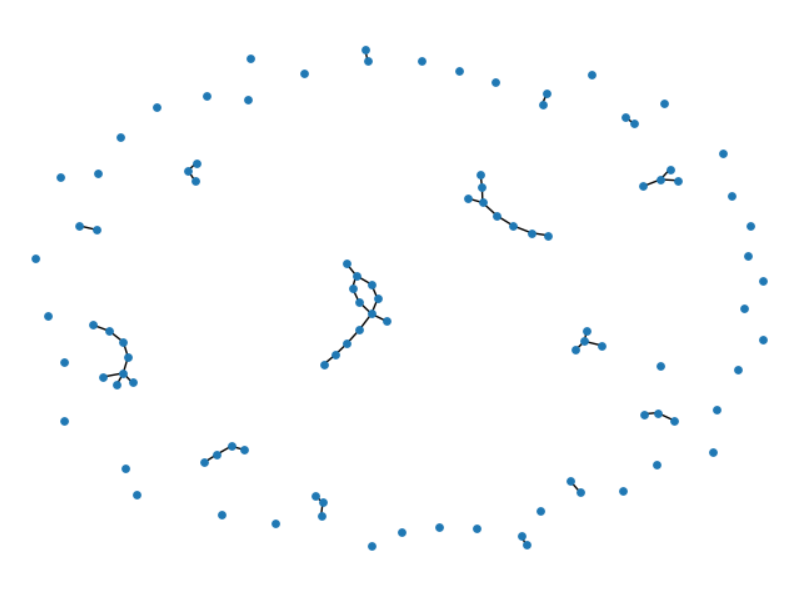
\includegraphics[width=\linewidth]{image/E_R_N100_p0,01.png}
    \end{subfigure}
    \hfill
    \begin{subfigure}[t]{0.49\textwidth}
        \centering
        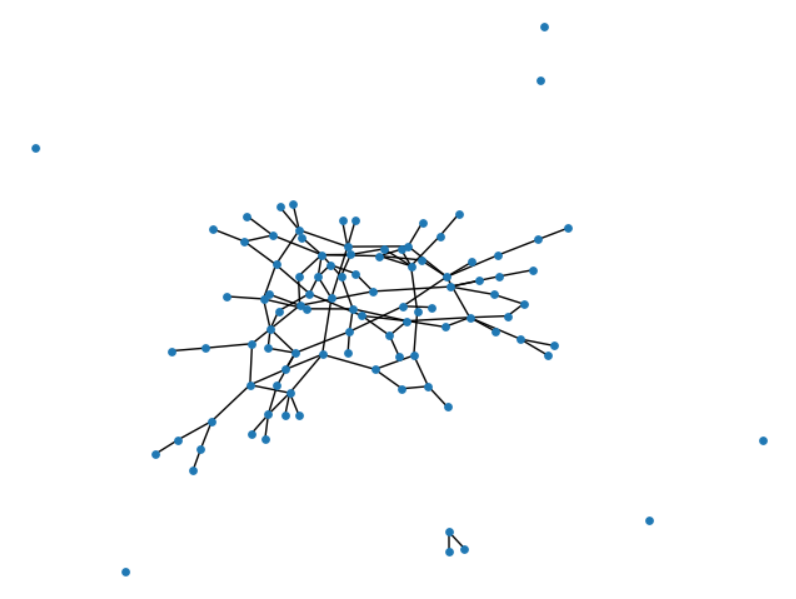
\includegraphics[width=\linewidth]{image/E_R_N100_p0,02.png}
    \end{subfigure}
    \caption{Two example of Erd\H{o}s-Rényi random graphs: on the left, it has 100 nodes and $p = 0.01$; on the right, it has 100 nodes and $p = 0.02$. Overcoming the threshold $p > 0.01$ can be seen the formation of the giant component.}
    \label{E-R_example}
\end{figure}
%the algorithm is define as below :
%\begin{enumerate}
 %   \item we identify the graph by its adjacency matrix;
 %   \item For each possible link, we generate a random number, if it is less than $p$ the respective entry in the adjacency matrix  is 1 otherwise 0.
%\end{enumerate}

However, the E-R algorithm do not produces network similar to the real ones found in nature, they tend to be more clustered and to have hubs (nodes with very high degree). To simulate this properties new algorithms have been proposed, like the Barab\'abi-Albert scale-free network and the Watts-Strogatz small world network.

\subsection{Barab\'abi-Albert scale-free network}
Barab\'abi and Albert proposed a scale-free Network $G(N, m)$ \cite{Barabasi_Albert_1999} that mimics the behavior of real graph like the Internet. This type of graph shows some preferential nodes which have a degree order of magnitude higher that the average and present a power law as degree distribution.
The model works by preferential attachment, where new nodes are more likely to connect to nodes that already have a higher degree. 

The algorithm is define below:
\begin{enumerate}
    \item It is initialized a complete graph of $m_0 > m$ node, usually $m_0 = m+1$;
    \item The other nodes are connected to this graph: for each new node, it is connected to $m$ nodes with probability $p_i = \frac{k_i}{\sum_i k_i}$, where $k_i$ is the degree of the $i$ node.
\end{enumerate}
In figure \ref{B-A_example} it is shown two example of B-A networks.

\begin{figure}[ht!]
    \centering
    \begin{subfigure}[t]{0.49\textwidth}
        \centering
        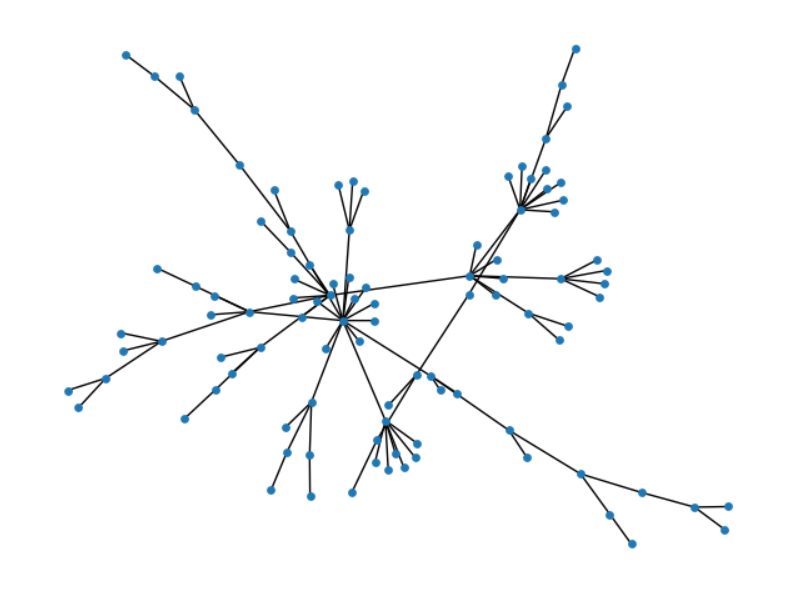
\includegraphics[width=\linewidth]{image/B_A_N100_m1.png}
    \end{subfigure}
    \hfill
    \begin{subfigure}[t]{0.49\textwidth}
        \centering
        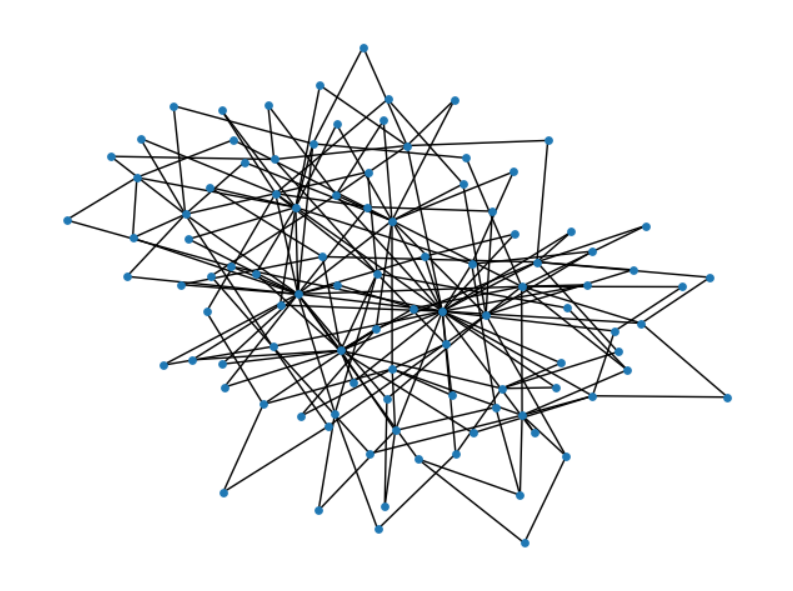
\includegraphics[width=\linewidth]{image/B_A_N100_m2.png}
    \end{subfigure}
    \caption{Two example of Barab\'abi-Albert scale-free networks: on the left, it has 100 nodes and $m=1$; on the right, it has 100 nodes and $m=2$.}
    \label{B-A_example}
\end{figure}

\subsection{Watts-Strogatz small world network}

The Watts-Strogatz small world network $G(N, K, p)$ \cite{Watts-Strogatz_1998}, where $N$ is the number of nodes, $K$ is the average degree (it must be even) and $p$ is the rewiring probability, is a model that exhibit high clustering and short average path lengths. The degree distribution is a power law and the network is homogeneous, all nodes have similar degree.

The algorithm is shown below:
\begin{enumerate}
    \item It is created a ring network with $N$ nodes where each node is connect to the $K/2$ nearest neighbors for each side;
    \item For each edge with probability $p$, the link is removed and another one to node chosen uniformly at random is created, the new link must be a not existing one.
\end{enumerate}

In figure \ref{W-S_example} it is shown two example of W-S networks.

\begin{figure}[ht!]
    \centering
    \begin{subfigure}[t]{0.49\textwidth}
        \centering
        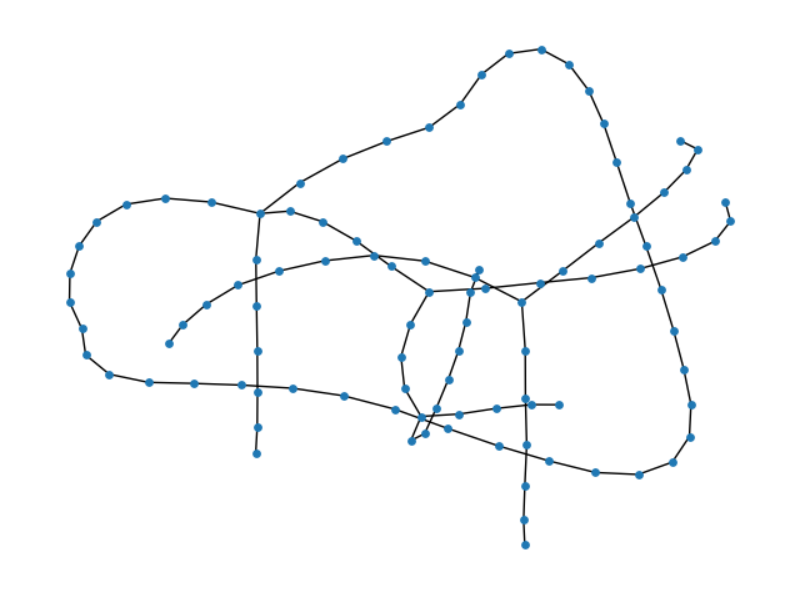
\includegraphics[width=\linewidth]{image/W_S_N100_K2_p0,1.png}
    \end{subfigure}
    \hfill
    \begin{subfigure}[t]{0.49\textwidth}
        \centering
        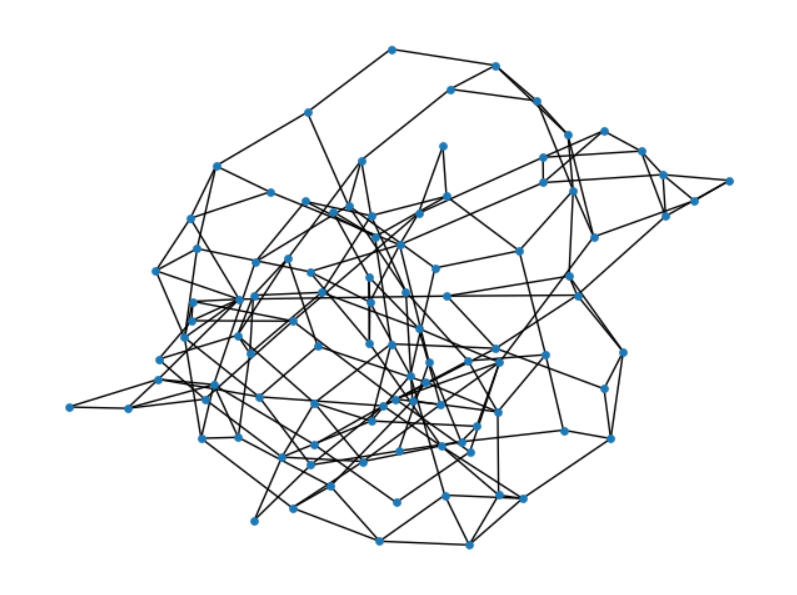
\includegraphics[width=\linewidth]{image/W_S_N100_K4_p0,3.png}
    \end{subfigure}
    \caption{Two example of Watts-Strogatz small world networks: on the left, it has 100 nodes, $K=2$ and $p=0.1$; on the right, it has 100 nodes, $K=4$ and $p=0.3$.}
    \label{W-S_example}
\end{figure}

The B-A and W-S algorithms produce more realistic networks respect to the E-R one, but both focus on their special feature: the B-A network fails to reproduce the high clustering of real network and the W-S one fails to reproduce the hubs  characteristic of scale-free networks.